\ifx\wholebook\relax \else

\documentclass[UTF8]{article}

%
% loading packages
%

\RequirePackage{ifpdf}
\RequirePackage{ifxetex}

\ifpdf
  \RequirePackage[pdftex,%
       bookmarksnumbered,%
              colorlinks,%
          linkcolor=blue,%
              hyperindex,%
        plainpages=false,%
       pdfstartview=FitH]{hyperref}
\else\ifxetex
  \RequirePackage[bookmarksnumbered,%
               colorlinks,%
           linkcolor=blue,%
               hyperindex,%
         plainpages=false,%
        pdfstartview=FitH]{hyperref}
\else
  \RequirePackage[dvipdfm,%
        bookmarksnumbered,%
               colorlinks,%
           linkcolor=blue,%
               hyperindex,%
         plainpages=false,%
        pdfstartview=FitH]{hyperref}
\fi\fi
%\usepackage{hyperref}

% other packages
%--------------------------------------------------------------------------
\usepackage{graphicx, color}
\usepackage{wrapfig}
\usepackage{subcaption}  %subfig is deprecated
\usepackage{multicol}
\usepackage[table]{xcolor} %for colored table
\usepackage{tikz}
\usetikzlibrary{patterns,matrix,positioning,shapes}

\usepackage{amsmath, amsthm, amssymb, amsbsy} % for math
\usepackage{textgreek, upgreek}
\usepackage{gensymb}
\usepackage{mathtools}
\usepackage{extarrows}
\usepackage{exercise} % for exercise
\usepackage{import} % for nested input

%
% for programming
%
\usepackage{verbatim}
\usepackage{fancyvrb}
\usepackage{listings}
\usepackage{algorithm} %to remove rules change to \usepackage[plain]{algorithm}
\usepackage[noend]{algpseudocode} %for pseudo code, include algorithmicsx automatically
\usepackage{appendix}
\usepackage{makeidx} % for index support
\usepackage{titlesec}
\usepackage{epigraph}

\usepackage{fontspec}
\usepackage{xunicode}
\usepackage{textcomp}
\usepackage{url}

% detect and select Chinese font
% ------------------------------
% fc-list :lang=zh    % list all Chinese fonts
% fc-list :mono       % list all mono fonts
% fc-cache            % refresh cache to load new installed fonts
\def\macmainfont{STSong}  % Under Mac OS X
\def\macmonofont{Monaco}
\def\winmainfont{SimSun} % Under Windows
\def\winmonofont{Consolas}
\def\linuxmainfont{WenQuanYi Micro Hei} % Under Linux
\def\linuxmainfont{Courier}

\suppressfontnotfounderror1 % Avoid setting exit code (error level) to break make process
\count255=\interactionmode
\batchmode

% main font
\let\cnmainft=\macmainfont
\font\thefont="\cnmainft"\space at 10pt
\ifx\thefont\nullfont
  \let\cnmainft=\winmainfont
  \font\thefont="\cnmainft"\space at 10pt
  \ifx\the\nullfont
    \let\cnmainft=\linuxmainfont
    \font\thefont="\cnmainft"\space at 10pt
    \ifx\the\nullfont
      \errorstopmode
      \errmessage{no suitable Chinese main font found}
    \fi
  \fi
\fi

% mono font
\let\monoft=\macmonofont
\font\thefont="\monoft"\space at 10pt
\ifx\thefont\nullfont
  \let\monoft=\winmonofont
  \font\thefont="\monoft"\space at 10pt
  \ifx\the\nullfont
    \let\monoft=\linuxmonofont
    \font\thefont="\monoft"\space at 10pt
    \ifx\the\nullfont
      \errorstopmode
      \errmessage{no suitable mono font found}
    \fi
  \fi
\fi

\interactionmode=\count255

\titleformat{\paragraph}
{\normalfont\normalsize\bfseries}{\theparagraph}{1em}{}
\titlespacing*{\paragraph}
{0pt}{3.25ex plus 1ex minus .2ex}{1.5ex plus .2ex}

% for literate Haskell code
\lstdefinestyle{Haskell}{
  flexiblecolumns=false,
  basewidth={0.5em,0.45em},
  morecomment=[l]--,
  literate={+}{{$+$}}1 {/}{{$/$}}1 {*}{{$*$}}1 {=}{{$=$}}1
           {>}{{$>$}}1 {<}{{$<$}}1 {\\}{{$\lambda$}}1
           {\\\\}{{\char`\\\char`\\}}1
           {->}{{$\rightarrow$}}2 {>=}{{$\geq$}}2 {<-}{{$\leftarrow$}}2
           {<=}{{$\leq$}}2 {=>}{{$\Rightarrow$}}2
           {\ .}{{$\circ$}}2 {\ .\ }{{$\circ$}}2
           {>>}{{>>}}2 {>>=}{{>>=}}2
           {|}{{$\mid$}}1
}

\lstloadlanguages{C, C++, Java, Lisp, Haskell, Python}

\lstset{
  basicstyle=\small\ttfamily,
  commentstyle=\rmfamily,
  texcl=true,
  showstringspaces = false,
  upquote=true,
  flexiblecolumns=false
}

\newcommand\doubleplus{+\kern-1.3ex+\kern0.8ex}

% ======================================================================


\def\BibTeX{{\rm B\kern-.05em{\sc i\kern-.025em b}\kern-.08em
    T\kern-.1667em\lower.7ex\hbox{E}\kern-.125emX}}

%
% mathematics
%
\newcommand{\be}{\begin{equation}}
\newcommand{\ee}{\end{equation}}
\newcommand{\bmat}[1]{\left( \begin{array}{#1} }
\newcommand{\emat}{\end{array} \right) }
\newcommand{\VEC}[1]{\mbox{\boldmath $#1$}}

% numbered equation array
\newcommand{\bea}{\begin{eqnarray}}
\newcommand{\eea}{\end{eqnarray}}

% equation array not numbered
\newcommand{\bean}{\begin{eqnarray*}}
\newcommand{\eean}{\end{eqnarray*}}

\newtheorem{theorem}{Theorem}[section]
\newtheorem{lemma}[theorem]{Lemma}
\newtheorem{proposition}[theorem]{Proposition}
\newtheorem{corollary}[theorem]{Corollary}
\newtheorem{definition}{Definition}[section]
\newtheorem{example}{Example}[section]

\makeatletter
\newcommand{\verbatimfont}[1]{\renewcommand{\verbatim@font}{\ttfamily#1}}
\makeatother

\setcounter{tocdepth}{4}
\setcounter{secnumdepth}{4}


\setcounter{page}{1}

\begin{document}

% ================================================================
%                 Digit lock
% ================================================================

\title{Natural Numbers}

\author{LIU Xinyu
\thanks{{\bfseries LIU Xinyu} \newline
  Email: liuxinyu95@gmail.com \newline}
  }

\maketitle
\fi

\markboth{Natural numbers}{Algebra of Computer Programming}

\epigraph{Numbers are the highest degree of knowledge. It is knowledge itself.}{--Plato}

\section{The history of number}

\begin{wrapfigure}{R}{0.3\textwidth}
%\begin{figure}[htbp]
 \centering
 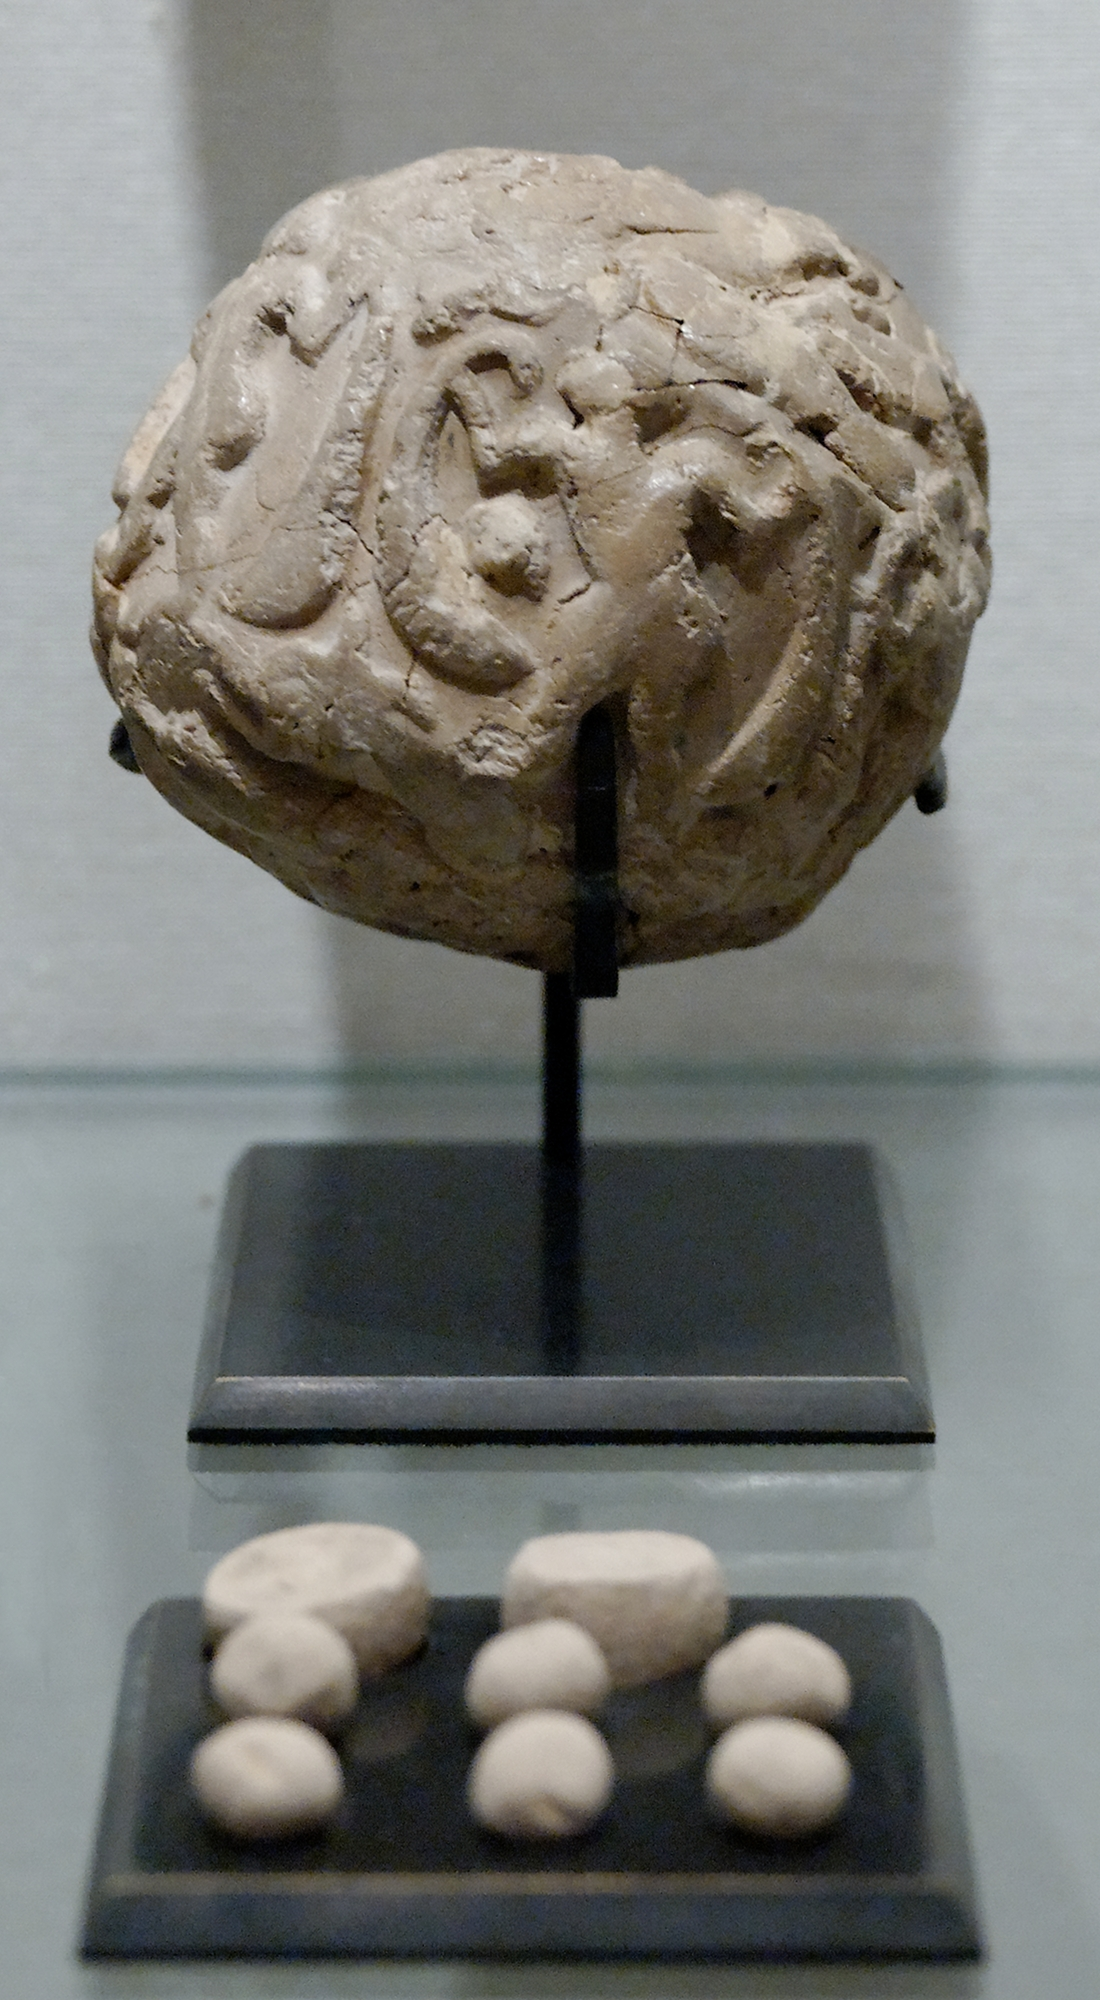
\includegraphics[scale=0.3]{img/clay-envelope.eps}
 \caption{The envelop of tokens in Uruk period from Susa. Louvre Museum}
 \label{fig:clay-token}
%\end{figure}
\end{wrapfigure}

The number emerged with human evolution. Some people beleive the language is inspired by number. Our ancestors learnt the numbers from the gathering and hunting activities. People need count the number of the fruits gathered. As the trading is developed, people need numeral tools to handle the bigger numbers than before.

We found in the regions of Iran, people use clay tokens for record keeping around 4000 BC. they created two round tokens with `+' sign baked to represent "two sheep". Each token represented one sheep. Representing a hundred sheep with a hundred tokens would be impractical, so they invented different clay tokens to represent ten sheep, ten goats and so on. In order to avoid the record being altered, people invented a clay envelope in which to tokens were placed, sealed, and baked. If anybody disputed the number, they could break open the clay envelope and do a recount. They also pressed the signs outside the envelop before it was baked, these signs on the outside became the first written language for writing numbers\cite{trip-to-number-kindom}. Figure \ref{fig:clay-token} shows the acient clay tokens and evelopes found in Uruk period.

As the number kept increasing, the clay tokens and evelops were gradually replaced by more powerful numerals. About 3500 BC, the Sumerians in Mesopotamia use round stylus in flat clay tablets to carve pictographs representing various tokens. Each sign represented both commodity being counted and the quantity of that commodity.

The next big step happend around 3100 BC. The abstract numbers dissociated from the thing being counted. We found from the clay tablets, the things being counted were indicated by pictographs carved with a sharp stylus next to round-stylus numerals. These abstracted numerals later evolved to the Babylonian cuneiform characters.

%\begin{wrapfigure}{R}{0.5\textwidth}
\begin{figure}[htbp]
 \centering
 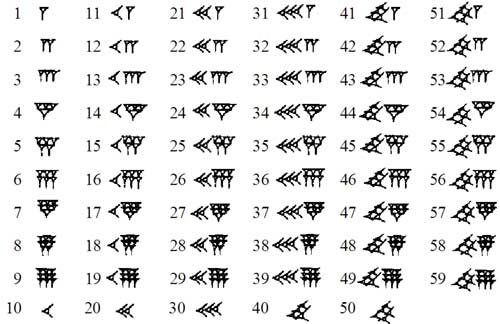
\includegraphics[scale=0.6]{img/Babylonian_numerals.eps}
 \caption{Babylonian numerals\cite{wiki-babylonian-num}。}
 \label{fig:babylonian-num}
\end{figure}
%\end{wrapfigure}

The abstract number is the emerged from intelligent mind. People realized the abstract number three could represent three eggs, three trees, and three jars. It's a powerful tool. People can manupulate the pure numbers, and apply the result on the concrete things. When increase the abstract three by one to get four, we know gathering another egg after three eggs gives four eggs; we also know baking another jar after three jars gives four jars. We resolve a whole kind of problem instead of one by one.

%\begin{wrapfigure}{R}{0.5\textwidth}
\begin{figure}[htbp]
 \centering
 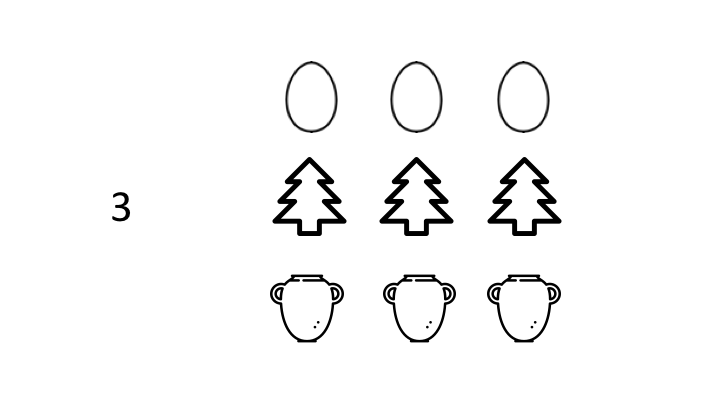
\includegraphics[scale=0.2]{img/abstract-num.eps}
 \caption{The concreate three things and the abstract three}
 \label{fig:abstract-num}
\end{figure}
%\end{wrapfigure}

Starting from the numbers, people developed add, substruction, then the more powerful method like multiplication and division. When measure the length, angles, areas, and volumes, we connected the number to the geometry. People from different acient places found the inner relationships and laws for the numbers and shapes. Acient Egypt, Greek, China found the Pythagoras theorem indeendantly, and applied it to the amazing works like to build the greate pyramid. Trace back from the modern civilization, we'll find the natural number is the source of math and science. Kronecker, a German mathematician said `God made the integers; all else is the work of man.'\footnote{Natual number is different from integer. We'll come back to the story of Kronecker in the chapter of infinity and Cantor.}


\section{Peano Axioms}

%\begin{wrapfigure}{R}{0.4\textwidth}
\begin{figure}[htbp]
 \centering
 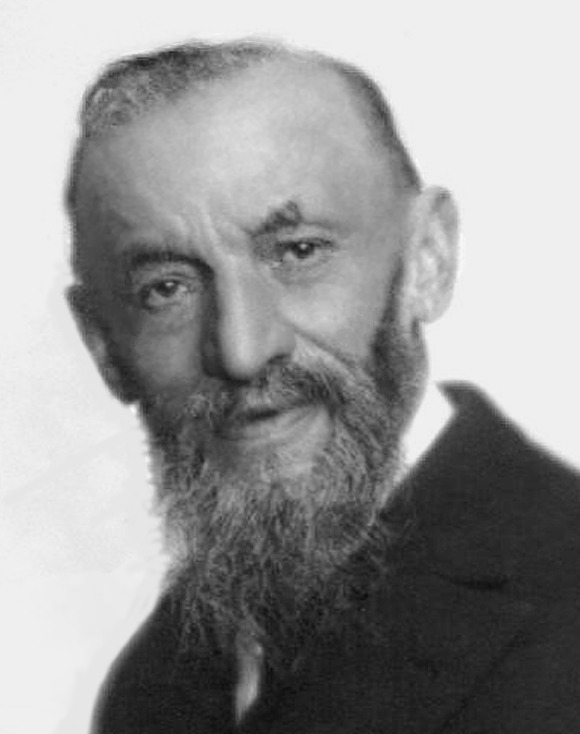
\includegraphics[scale=0.2]{img/Peano.eps}
 \caption{Giuseppe Peano (1858-1932)}
 \label{fig:Peano}
\end{figure}
%\end{wrapfigure}

Euclid's Element is the first work introduced the axiomatic methods. From the five axioms and five postulates, Euclid developed the laws one by one elaborately. Every result is only based on the axioms and the laws proven before. With this approach, he built the great building of geometry. However, theres no axiomatic formal system for natural numbers for long time compare to the geometry. People have been considering the natural number is straightforward and the related facts are obvious. The axioms of natural number was setup by Italian mathematics Peano till 1889\footnote{Peano is mathematician, logician, and linguist. He is the poineer of mathematical logic and set theory. Peano influenced Russel and Whitehead for their work `Principia Mathematica', and the further programs of French Bourbaki school. Peano also invented an international auxiliary language called Latino sine flexione ("Latin without inflexion," later called Interlingua, and the precursor of the Interlingua of the IALA).}. Today, we called Peano Axioms. It may be arranged by God, similiar to Euclid's five geometry axioms, there are five Peano natural number axioms.

\begin{enumerate}
\item 0 is a natural number. It can be expressed as $\exists 0 \in N$;
\item For every natural number, there is a successor natural number. Expressed as $\forall n \in N, \exists n' = succ(n) \in N$;
\end{enumerate}

It seems that we can define the infinite natural numbers only with these two axioms. From 0, the next is 1, then the next is 2, then 3, ..., then the next is $n$, then $n+1$, ..., till infinity. However, there is a counter example. Consider the number system consists of only two numbers $\{0, 1\}$. Where the successor of 1 is defined as 0, while the successor of 0 is defined as 1. It satisfies the above two axioms well although this isn't the natural number as we expected.

In order to avoid this situation, we need the third Peano axiom.

\begin{enumerate}
  \setcounter{enumi}{2}
  \item 0 isn't the successor of any natural number. Expressed as $\forall n \in N: n' \neq 0$;
\end{enumerate}

Are these three axioms enough? We can still find another counter example. Consider a finite number system with elements $\{0, 1, 2\}$. Define the successor of 0 is 1, the successor of 1 is 2, and the successor of 2 is 2 again. It can satisfy all the three axiom so far. We therefore need the fourth Peano axiom.

\begin{enumerate}
  \setcounter{enumi}{3}
  \item Different natural numbers have different successors. In other words, if two natural numbers have the same successor, then they are same. It can be formally expressed as $\forall n, m \in N: n' = m' \Rightarrow n = m$;
\end{enumerate}

It is not enough to only have these four axioms however. We can still find such example set of $\{0, 0.5, 1, 1.5, 2, 2.5, ...\}$. Define 1 is the successor of 0, 2 is the successor of 1, ...; 1.5 is the successor of 0.5, 2.5 is the successor of 1.5, ...; But 0.5 is not the successor of any other numbers. In order to exclude such `unreachable' elements, we need the last Peano axiom.

\begin{enumerate}
  \setcounter{enumi}{4}
  \item If some subset of natural numbers contains 0, and every element in it has successor, then this subset is same as the whole natural numbers. It can be expressed as $\forall S \subset N: (0 \in S \land \forall n \in S \Rightarrow n' \in S) \Rightarrow S = N$.
\end{enumerate}

Why does the fifth axiom exclude the above counter example? For $\{$0, 0.5, 1, 1.5, 2, 2.5, ...$\}$, consider the subset of $\{0, 1, 2, ...\}$. 0 is in it, and every element has successor. But it is not identity to the original set. As 1.5, 2.5, ... are not in this subset, it does not satisfy the fifth axiom. This last axiom as also known as `Axiom of induction'. It can be equally stated as the following.

\begin{enumerate}
  \setcounter{enumi}{4}
  \item For any proposition of natural numbers, if it holds for 0, and when assume it holds for some number $n$, we can prove it also holds for $n'$, then the propostion holds for all natural numbers. (This axiom ensure the correctness of mathematical induction.)
\end{enumerate}

This the complete statement of the five Peano axioms. They can build the first-order arithmetic, also known as Peano arithmetic\footnote{Some people use 1, but not 0 as the first natural number. The order is different from the orignial works published by Peano, where the fifth axiom of induction was list as the third one.}.

\section{Natual numbers and programming}

People make amazing achievement with the modern computer systems and the programs. We didn't establish the axioms of computer programming before developing these results. After the great success of computer application, then the foundation of computer science is gradually developed to be strict, formal, and mathematized. The similiar thing happens several times in our history. Calculus was developed by Newton and Leibniz indenpendantly in the 17th centry, then applied to a wide range of areas, including fluid dynamics, astronomy and so on. However, it was not formalized until Cauchy developed it's foundation in the 19th centry.

We'll emulate it. From the Peano axioms, define the natural numbers with computer programs. In a computer system without familiar numbers like 0, 1, 2, ..., we can define the natural numbers as below\footnote{We use a virtual, ideal programming language in this book. Some real programs are given at the end of each chapter for reference.}:

\lstset{language=Haskell}
\begin{lstlisting}
data Nat = zero | succ Nat
\end{lstlisting}

%% \[
%% N \triangleq zero | succ(N)
%% \]

A natural number is either zero, or the successor of another natural number. Symbol `|' is mutual exclusive, it implicates the axiom that zero is not the successor of any natural number. We can further define the addition for natural numbers with this definition.

\begin{lstlisting}
a + zero = a
a + (succ b) = succ (a + b)
\end{lstlisting}

There are two rules for addition. First, any natural number adds zero gives that number itself; second, a natural number adds to a successor of some natual number equals to the successor of the sum of these two numbers. In mathematic expression:

\be
\begin{array}{l}
a + 0 = a \\
a + b' = (a + b)'
\end{array}
\ee

Let's use 2+3 as the example. natural number 2 is succ(succ zero), and 3 is succ(succ(succ zero)). According to the definition of addition:

\begin{lstlisting}
  succ(succ zero) + succ(succ(succ zero))
= succ(succ(succ zero) + succ(succ zero))
= succ(succ(succ(succ zero) + succ zero))
= succ(succ(succ(succ(succ zero) + zero)))
= succ(succ(succ(succ(succ zero))))
\end{lstlisting}

The result is the 5th successor of zero. It's not practical to apply succeed function again and again when express big numbers like 100. Let's introduce a simplified notation for natural number $n$.

\be
n = foldn(zero, succ, n)
\ee

It applies $succ$ function on zero $n$ times. Function $foldn$ can be realized as the following.

\be
\begin{array}{l}
foldn(z, f, 0) = z \\
foldn(z, f, n') = f(foldn(z, f, n))
\end{array}
\label{eq:foldn}
\ee

Function $foldn$ defines some operation on natural number. When let $z$ is $zero$, and $f$ is the $succ$ function, then it can apply the succeed operation multiple times to get a specific natural number. We can verify it with the first several natural numbers.

\begin{lstlisting}
foldn(zero, succ, 0) = zero
foldn(zero, succ, 1) = succ(foldn(zero, succ, 0)) = succ zero
foldn(zero, succ, 2) = succ(foldn(zero, succ, 1)) = succ(succ zero)
...
\end{lstlisting}

Multiplication for natural number can be defined on top of addition.

\begin{lstlisting}
a . zero = zero
a . (succ b) = a . b + a
\end{lstlisting}

It reuses the addition defined above. The mutliplication can be expressed in mathematic symbols as below.

\be
\begin{array}{l}
a \cdot 0 = 0 \\
a \cdot b' = a \cdot b + a
\end{array}
\ee

\begin{wrapfigure}{R}{0.4\textwidth}
\centering
\begin{tikzpicture}[scale=0.8]
\filldraw[fill=gray, draw=black, pattern=north west lines] (0, 0) rectangle (2, 1)
    (2, 0) rectangle (3, 1);
\draw (3, 0) rectangle (4.5, 1);
\draw (0, -1) rectangle (2, -2);
\filldraw[fill=gray, draw=black, pattern=north west lines] (2, -1) rectangle (3, -2)
    (3, -1) rectangle (4.5, -2);
\end{tikzpicture}
\caption{Association of addition in geometry. The above and bottom areas are same.}
\end{wrapfigure}

It turns out that the associative and commutative laws for addition and multiplication are neigher axioms nor postulations. They all can be proven by Peano axioms and the defintions. Let's prove the associative law for addition as an example. This law states that $(a + b) + c= a + (b + c)$. We firstly prove it holds when $c=0$. According to the first rule in the add definition:

\[
\begin{array}{rl}
(a + b) + 0 & = a + b \\
            & = a + (b + 0)
\end{array}
\]

Then for induction, assume $(a + b) + c = a + (b + c)$ hold, we want to deduce $(a + b) + c' = a + (b + c')$.

\[
\begin{array}{rlr}
(a + b) + c' & = (a + b + c)' & \text{2nd equation defining +, (backwards)} \\
             & = (a + (b + c))' & \text{induction assumption} \\
             & = a + (b + c)' & \text{2nd equation defining +} \\
             & = a + (b + c') & \text{2nd equation defining +, (backwards)}
\end{array}
\]

This complete the proof of associative law for addition. However, it is a bit complex to prove the commutative law. We give it in Appendix I.

%\begin{wrapfigure}{R}{0.4\textwidth}
\begin{figure}[htbp]
\centering
\begin{tikzpicture}[scale=0.8]
\draw (0, 0) rectangle (2, 1)
    (2, 0) rectangle (3, 1);
\draw (0, -1) rectangle (1, -2)
    (1, -1) rectangle (3, -2);
\end{tikzpicture}
\caption{Commutative law of addition in geometry. Turn upside down or mirrow the upper figure.}
\end{figure}
%\end{wrapfigure}

\begin{Exercise}
\begin{enumerate}
\item Define 1 as the successor of 0, prove $a \cdot 1 = a$ hold for all natural numbers;
\item Prove the associative and commutative laws for multiplication;
\item Prove the distributive law for multiplication.
\end{enumerate}
\end{Exercise}

\section{Structure of natural numbers}

We can define more complex operations on top of addition and multiplication. One example is summation: $0 + 1 + 2 + ... $

\be
\begin{array}{l}
sum(0) = 0 \\
sum(n + 1) = (n + 1) + sum(n)
\end{array}
\ee

Another example is the fraction $n!$

\be
\begin{array}{l}
fact(0) = 1 \\
fact(n + 1) = (n + 1) \cdot fact(n)
\end{array}
\ee

They are similiar to each other. Although artificial intelligence achieves incredible result today, the machine can't jump out of the system as intelligent life, to abstract in a higher level. This is one of the most complex, powerful, mysterious part in human mind\cite{GEB}.

Corresponding to zero in natural number, both summation and fraction have a start value. Summation starts from zero, fraction starts from one. For recurssion, they both apply some operation on a number and its successor. For summation, it's $n' + sum(n)$, for fraction, it's $n' \cdot fact(n)$. If we abstract the start value as $c$, the recursive operation as $h$, then we can use a same form for both summation and fraction.

\be
\begin{array}{l}
f(0) = c \\
f(n + 1) = h(f(n))
\end{array}
\ee

This scheme is called definition by {\em structural} recursion over the natural numbers. Below examples show how it behaves over the first
 several numbers.

\begin{tabular}{l|l}
$n$ & $f(n)$ \\
\hline
0 & $c$ \\
1 & $f(1) = h(f(0)) = h(c)$ \\
2 & $f(2) = h(f(1)) = h(h(c))$ \\
3 & $f(3) = h(f(2)) = h(h(h(c)))$ \\
... & ... \\
$n$ & $f(n) = h^n(c)$
\end{tabular}

Where $h^n(c)$ means applying operation $h$ over $c$ for $n$ times. It's an instance of a more general {\em primitive} recursion(\cite{Bird97}, p5). Further, we can find the relation to the $foldn$ defined in (\ref{eq:foldn}).

\be
f = foldn(c, h)
\ee

Why there are three variables in the original $foldn$ definition, while there are only two here? We can actually write it as $f(n) = foldn(c, h, n)$. When we bind the first two variables to $foldn$, it turns to be a new function accepts one argument. We can consider it as $foldn(c, h)(n)$.

We call $foldn$ is the {\em fold} operation on natural numbers. When $c$ is $zero$ and $h$ is $succ$, we get a sequence of natural numbers:

\[
zero, succ(zero), succ(succ(zero)), ... succ^n(zero), ...
\]

When $c$ and $h$ are other things than $zero$ or $succ$, then $foldn(c, h)$ describe some isomorphism\footnote{The formal definition of isomorphism will be given in later chapters. Different from the methematic definition, here it means a similarity in terms of pattern.} to natural numbers. Here are some examples.

\[
(+ m) = foldn(m, succ)
\]

This is the operation to increase a number by $m$. Whey applying to the natural numbers, it generates an isomorphic sequence of $m, m + 1, m + 2, ..., n + m, ...$

\[
(\cdot m) = foldn(0, (+ m))
\]

This is the operation to multiply a number by $m$. Whey applying to the natural numbers, it generates an isomorphic sequence of $0, m, 2m, 3m, ..., nm, ...$

\[
m^{()} = foldn(1, (\cdot m))
\]

This is the operation to take the power for a number $m$. Whey applying to natural numbers, it generates an isomorphic sequence of $1, m, m^2, m^3, ..., m^n, ...$

Can we use the abstract tool $foldn$ to define summation and fraction? Observe the below table.

\begin{tabular}{r|l|l|l|l|l|l}
$n$ & 0 & 1 & 2 & 3 & ... & $n'$ \\
\hline
$sum(n)$ & 0 & 1 + 0 = 1 & 2 + 1 = 3 & 3 + 3 = 6 & ... & $n' + sum(n)$ \\
\hline
$n!$ & 1 & 1 $\times$ 1 = 1 & 2 $\times$ 1 = 2 & 3 $\times$ 2 = 6 & ... & $n' \cdot (n!)$
\end{tabular}

We know that $h$ need to be a binary operation as it manipulates $n'$ and $f(n)$. To solve it, we define $c$ as a pair $(a, b)$\footnote{Also known as {\em tuple} in computer programs}. Then define some kind of `succ' operation on the pair. We also need functions to extract $a$ and $b$ from the pair.

\be
\begin{array}{l}
1st (a, b) = a \\
2nd (a, b) = b
\end{array}
\ee

With these setup, we can define summation:

\[
\begin{array}{ll}
c = (0, 0) & \text{Starting pair} \\
h (m, n) = (m', m' + n) & \text{Succeed the 1st; Add the 2nd and the successor} \\
sum = 2nd \cdot foldn(c, h) \\
\end{array}
\]

Starting from $(0, 0)$, below table gives the steps for summation.

\begin{tabular}{r|l|l}
$(a, b)$ & $(a', b') = h (a, b)$ & $b'$\\
\hline
(0, 0) & (0 + 1 = 1, 1 + 0 = 1) = (1, 1) & 1 \\
(1, 1) & (1 + 1 = 2, 2 + 1 = 3) = (2, 3) & 3 \\
(2, 3) & (2 + 1 = 3, 3 + 3 = 6) = (3, 6) & 6 \\
... & ... & ... \\
$(m, sum(m))$ & $(m + 1, m + 1 + sum(m))$ & $sum(m + 1)$
\end{tabular}

Similiarily, we can define fraction with $foldn$.

\[
\begin{array}{lr}
c = (0, 1) & \text{Starting pair for fraction} \\
h (m, n) = (m', m'n) & \text{Iteration for fraction} \\
fact = 2nd \cdot foldn(c, h) \\
\end{array}
\]

Here we use the symbol `$\cdot$' to `connect' the $2nd$ function and the $foldn(c, h)$ function. We call it {\em function composition}. $f\cdot g$ means first apply $g$ to the variable, then apply $f$ on top of the result. That is $(f\cdot g)(x) = f(g(x))$.

\begin{wrapfigure}{R}{0.4\textwidth}
%\begin{figure}[htbp]
 \centering
 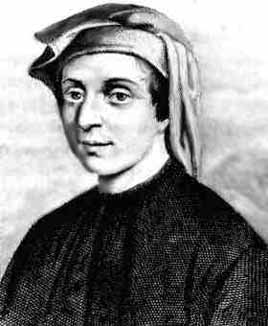
\includegraphics[scale=0.4]{img/Fibonacci.eps}
 \caption{Leonardo Pisano, Fibonacci (1175-1250)}
 \label{fig:abstract-num}
%\end{figure}
\end{wrapfigure}

Let's see another example powered by this abstract tool, Fibonacci sequence. It's named after the midieval mathematician Leonardo Pisano. Fibonacci originates from `filius Bonacci' in Lattin. It means the son of (the) Bonacci. Fibonacci's father was a wealthy Italian merchant
 often did trading around North Africa and the Mediterranean coast. Fibonacci travelled with him as a young boy. It was in Bugia (now Béjaïa, Algeria) that he learned about the Hindu–Arabic numeral system. Fibonacci realized the many advantage of this numeral system. He introduced it to Europe through his book, the Liber Abaci (Book of Abacus or Book of Calculation, 1202). European people was using Roman numeral system before that. Roman numbers stil can be seen in clock plat today. The Roman number for year 2018 is MMXVIII. Where an M for 1000, so two Ms mean 2000; X represents for 10, V for 5, the three I means 3. Sum them up, we get 2018. The Hindu-Arabic numeral system introduced by Fibonacci is a positional decimal numeral system we are using today. It uses the zero invented by Indian mathematicians. Numbers at different position means differnet value. This advanced numeral system were widely used in business, for example converting different currencies, and calculating profit and interest, which were important to the growing banking industry. It influenced the mathematics in Europe greatly.

Fibonacci numbers was a problem described in the Libe Abaci, although it can be traced back to 200BC in India. assuming that: a newly born pair of rabbits, one male, one female, are put in a field; rabbits are able to mate at the age of one month so that at the end of its second month a female can produce another pair of rabbits; rabbits never die and a mating pair always produces one new pair (one male, one female) every month from the second month on. The puzzle that Fibonacci posed was: how many pairs will there be in one year?

斐波那契数列来自《算盘书》中的一个问题:兔子在出生两个月后,就有繁殖能力,一对兔子每个月能生出一对小兔子来。如果所有兔都不死,那么一年以后可以繁殖多少对兔子?开始时有一对兔子。第一个月小兔尚未具备繁殖能力,所以仍然只有一对兔子。第二个月它们生下一对小兔,共有两对。第三个月大兔子又生下一对小兔,而上月生的小兔还在成长,总共有2+1=3对。第四个月有两对大兔子产下两对小兔,加上原有的三对兔子,总共有3+2=5对。按照这样,我们可以得到一个序列

1, 1, 2, 3, 5, 8, 13, 21, 34, 55, 89, 144, ...

\begin{wrapfigure}{L}{0.3\textwidth}
%\begin{figure}[htbp]
 \centering
 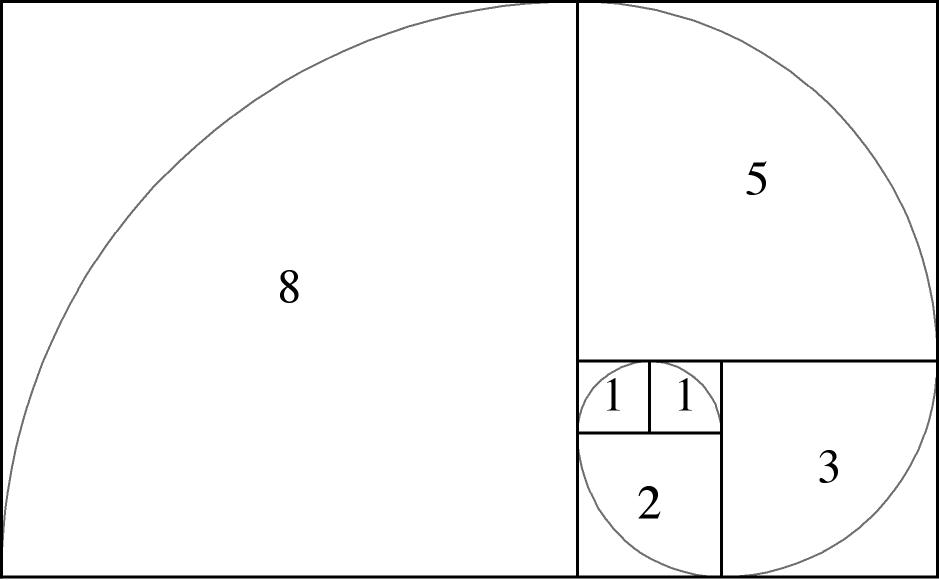
\includegraphics[scale=0.2]{img/fibonacci_spiral.eps}
 \caption{这些正方形的边长组成了斐波那契序列。}
 \label{fig:fibonacci_spiral}
%\end{figure}
\end{wrapfigure}

这个数列很有规律,从第三项后,任何一项都等于前两项的和。我们可以这样思考它的原理,如果前一个月有$m$对兔子,这个月有$n$对兔子,那么增加的一定都是新产下的小兔,共有$n-m$对,而剩下的都是成年兔子,共$m$对。到下个月时,这$n-m$对小兔刚刚成熟,而$m$对成兔又产下了$m$对小兔。所以下个月的兔子总数等于小兔加上成兔为:$(n - m) + m + m = n + m$对。根据这一推理,我们可以给出斐波那契数列的递归定义:

\be
\begin{array}{l}
F_0 = 0 \\
F_1 = 1 \\
F_{n+2} = F_n + F_{n+1}
\end{array}
\ee

习惯上通常将斐波那契数列的起始值定义为0和1\footnote{如果起始值是1和3,我们就得到了卢卡斯数列1, 3, 4, 7, 11, 18, ...}。注意到斐波那契数列的起始值是一对自然数,并且递推关系也是一对值。我们可以利用抽象工具$foldn$给出下面的定义\footnote{在介绍康托尔的无穷概念时,我们会给出另一个斐波那契数列的定义。}:

\be
\begin{array}{l}
F = 1st \cdot foldn((0, 1), h) \\
h (m, n) = (n, m + n)
\end{array}
\ee

也许读者会好奇,真实的计算机程序能实现这样的定义么?这是不是太理想化了?下面方框是一段的Haskell语言的程序代码\footnote{2010年后,Haskell中不再允许使用n+k形式的模式匹配,可以修改为:\newline\texttt{foldn z f n = f (foldn z f (n - 1))}},执行\texttt{fib 10}会输出斐波那契数55\footnote{一行代码输出前100个斐波那契数的例子:\newline\texttt{take 100 \$ map fst \$ iterate ($\lambda$(m, n)->(n, m + n)) (0, 1)}}。

\lstset{frame=single}
\begin{lstlisting}
foldn z _ 0 = z
foldn z f (n + 1) = f (foldn z f n)

fib = fst . foldn (0, 1) h where
  h (m, n) = (n, m + n)
\end{lstlisting}

\begin{Exercise}
\begin{enumerate}
\item 使用$foldn$定义$()^m$,计算给定自然数的$m$次幂。
\item 使用$foldn$定义平方。
\item 使用$foldn$定义奇数的平方和。它会产生怎样的序列?
\item 地面上有一排洞,一只狐狸藏在某个洞中。每天狐狸会移动到相邻的洞里。如果每天只能检查一个洞,请给出一个捉到狐狸的策略,并证明这个策略有效\cite{Gusen2014}。
\end{enumerate}
\end{Exercise}

%\begin{wrapfigure}{R}{0.3\textwidth}
\begin{figure}[htbp]
 \centering
 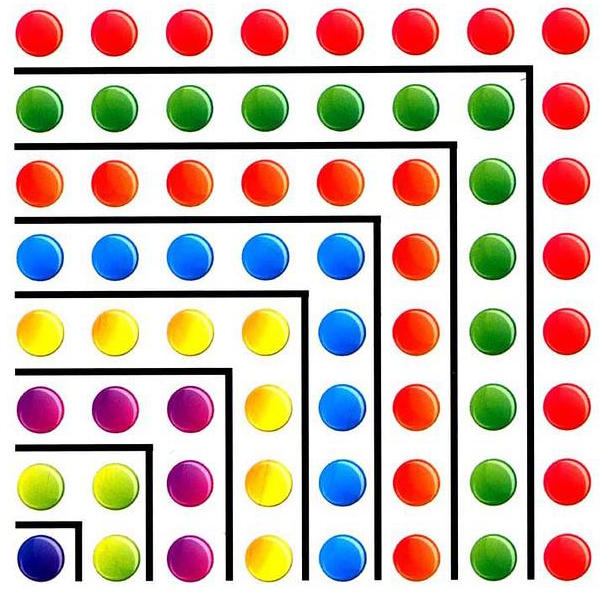
\includegraphics[scale=0.2]{img/PWW.eps}
 \caption{《无需语言的证明》封面局部}
 \label{fig:PWW}
\end{figure}
%\end{wrapfigure}

\section{自然数的同构}

自然数不仅可以和自己的子集同构,例如奇偶数、平方数、斐波那契数,还可以和其他事物同构。其中一个例子是计算机程序中的数据结构。下面是列表的定义:

\lstset{frame=none}
\begin{lstlisting}
data List A = nil | cons(A, List A)
\end{lstlisting}

用数据结构的观点来解释,一个类型为A的列表或者为空,记为nil;或者包含两部分:一个含有类型A数据的节点,和一个包含剩余部分的子列表。函数cons把一个类型为A的元素和另一个类型为A的列表“链接”起来\footnote{名称cons来自Lisp的命名传统。}。图\ref{fig:linked-list}描述了一个含有6个节点的列表。

\begin{figure}[htbp]
\centering
\begin{tikzpicture}[scale=3]
  \foreach \x in {-2, -1.7, ..., -0.4} {
    \draw (\x cm, 1cm) +(-0.1, -0.1) rectangle ++(0.1, 0.1);
    \draw[->] (\x cm, 1cm) +(0.05, 0) -- +(0.2, 0);
  }
  \draw (-0.2cm, 1cm) node {nil};
\end{tikzpicture}
\caption{Linked-list}
\label{fig:linked-list}
\end{figure}

由于这种特点,列表也被称为“链表”。传统的计算机程序中,链表通常定义为一个结构\footnote{很多情况下,列表中保存的数据类型是相同的。但也有异构类型的列表,例如Lisp中的列表。},例如:
\begin{verbatim}
Node of A:
    key: A
    next: Node of A
\end{verbatim}

我们也可以用自然数的同构来解释列表。根据皮亚诺公理一,nil相当于零;根据皮亚诺公理二,对于任何列表,我们都可以用cons,在其左侧链接一个类型为A的新元素。因此cons相当于自然数中的succ。这里的变化有两点。其一是列表携带类型A的元素,因而\texttt{cons(1, cons(2, cons(3, nil)))}和\texttt{cons(2, cons(1, cons(3, nil)))}和\texttt{cons(1, cons(4, cons(9, nil)))}以及\texttt{cons('a', cons('b', cons('c', nil)))}都是不同的列表。其二是与直觉不同,新元素不是加入到列表的右侧末尾,而是加入到左侧的头部。增长的方向是向左,而非向右。

用嵌套的cons表示较长的列表很不方便,我们将\texttt{cons(1, cons(2, cons(3, nil)))}简记为[1, 2, 3],用符号“:”表示cons。因此这一列表也可以写为1:[2, 3]或者1:(2:(3:nil))。针对A为字母的特殊情况,我们用带双引号的字符串来表示,例如用“hello”来简记表示['h', 'e', 'l', 'l', 'o']。

同构于自然数的加法,定义列表的连接运算如下:

\be
\begin{array}{l}
nil \doubleplus y = y \\
cons(a, x) \doubleplus y = cons(a, x \doubleplus y)
\end{array}
\ee

列表的连接运算包含两条规则。首先空列表和任何列表连接的结果仍然等于该列表本身;并且某个列表的“后继”和另一个列表相连接,等于这两个列表连接结果的后继。和自然数的加法对比,它们呈现出有趣的镜像对称形式。

\begin{figure}[htbp]
\begin{tabular}{r|l}
$nil \doubleplus y = y$ & $a + 0 = a$ \\
$cons(a, x) \doubleplus y = cons(a, x \doubleplus y)$ & $a + succ(b) = succ(a + b)$
\end{tabular}
\caption{列表的连接和自然数的加法呈现镜像对称}
\end{figure}

这种同构提示我们,可以利用递推公理证明列表连接的结合律。为了证明$(x \doubleplus y) \doubleplus z = x \doubleplus (y \doubleplus z)$,我们首先证明$x=nil$时的起始情况

\[
\begin{array}{lll}
(nil \doubleplus y) \doubleplus z & = y \doubleplus z & \text{列表连接定义的规则一} \\
 & = nil \doubleplus (y \doubleplus z) & \text{列表连接定义的规则一}
\end{array}
\]

然后再证明递推情况。假设$(x \doubleplus y) \doubleplus z = x \doubleplus (y \doubleplus z)$,我们要证明$((a:x) \doubleplus y) \doubleplus z = (a:x) \doubleplus (y \doubleplus z)$。

\[
\begin{array}{rll}
((a:x) \doubleplus y) \doubleplus z & = (a:(x \doubleplus y)) \doubleplus z & \text{列表连接定义的规则二} \\
 & = a:((x \doubleplus y) \doubleplus z) & \text{列表连接定义的规则二} \\
 & = a:(x \doubleplus (y \doubleplus z)) & \text{递推假设} \\
 & = (a:x) \doubleplus (y \doubleplus z) & \text{列表连接定义的规则二}
\end{array}
\]

这样我们就证明了列表连接操作的结合律。但是和自然数不同,列表不满足交换律\footnote{这也是我们避免使用加号“+”来表示列表连接的原因。但是很多编程语言使用了加号,这造成了一些潜在的问题。}。例如$[2, 3 ,5] \doubleplus [7, 11] = [2, 3, 5, 7, 11]$,但交换后的结果却是$[7, 11] \doubleplus [2, 3, 5] = [7, 11, 2, 3, 5]$。

考虑和自然数同构,我们也可以定义列表的抽象叠加操作。为此,我们仿照自然数定义一个抽象的起始值$c$,和一个抽象的二元运算$h$。这样就可以定义列表的递归形式:

\be
\begin{array}{l}
f(nil) = c \\
f(cons(a,x)) = h(a, f(x))
\end{array}
\ee

进一步,令$f = foldr(c, h)$,就可以抽象出列表的叠加操作。我们将其命名为$foldr$以表明这种叠加操作是从右侧开始,自右向左进行的。

\be
\begin{array}{l}
foldr(c, h, nil) = c \\
foldr(c, h, cons(a,x)) = h(a, foldr(c, h, x))
\end{array}
\ee

使用$foldr$,我们可以定义各种列表上的操作。例如我们可以把一个列表中的各个元素累加或累乘起来:

\be
\begin{array}{l}
sum = foldr(0, +) \\
product = foldr(1, \times)
\end{array}
\ee

我们可以通过一些例子了解$sum$的行为。首先是空列表:$sum([]) = foldr(0, +, nil) = 0$;然后是若干个元素的列表:

\[
\begin{array}{rl}
sum([1, 3, 5, 7]) & = foldr(0, +, 1:[3, 5, 7]) \\
 & = 1 + foldr(0, +, 3:[5, 7]) \\
 & = 1 + (3 + foldr(0, +, 5:[7])) \\
 & = 1 + (3 + (5 + foldr(0, +, cons(7, nil)))) \\
 & = 1 + (3 + (5 + (7 + foldr(0, +, nil)))) \\
 & = 1 + (3 + (5 + (7 + 0))) \\
 & = 16
\end{array}
\]

在$sum$的基础上,我们可以计算列表的长度。这本质上是把一个列表映射成自然数。

\be
\begin{array}{l}
one(a) = 1 \\
length = sum \cdot foldr(0, one)
\end{array}
\ee

其中函数$one$被称为“常数函数”,不管传入什么内容,它总返回常数1。这样我们就可以用$|x| = length(x)$来计算列表的长度。我们还可以用$foldr$定义连接操作$\doubleplus$:

\be
\doubleplus y = foldr(y, cons)
\ee

这相当于自然数的$(+m)$运算,类似自然数的乘法运算,我们可以定义列表的“乘法”,将一个列表的列表全部连接起来。

\be
concat = foldr(nil, \doubleplus)
\ee

例如:$concat([[1, 1], [2, 3, 5], [8]])$的结果是$[1, 1, 2, 3, 5, 8]$。我们接下来再用$foldr$定义两个列表的重要操作:选择和逐一映射\footnote{和一一映射不同,这里的映射是单向的,例如从一个词语到它的字符长度的映射,其逆映射并不存在。}。选择也称为过滤,是根据某个条件选择列表中的元素组成一个新的列表。为此,我们需要引入条件表达式的概念\footnote{也称麦卡锡条件形式,是计算机科学家Lisp发明人约翰$\cdot$麦卡锡于1960年引入的。}。它通常写为$(p \mapsto f, g)$,也就是给定变量$x$,若条件$p(x)$成立,则结果为$f(x)$,否则为$g(x)$,我们也会用if $p(x)$ then $f(x)$ else $g(x)$来描述条件表达式。

\be
filter(p) = foldr(nil, (p \cdot 1st \mapsto cons, 2nd))
\ee

为了理解这一定义,我们来看一个列子:从一组自然数中,选择出偶数,$filter(even, [1, 4, 9, 16, 25])$。和$sum$的例子类似,首先是一系列的展开过程,$h(1, h(4, h(9, ...)))$直到列表的最右侧$cons(25, nil)$。根据$foldr$的定义,传入$nil$的结果为$c$,故而接下来,要计算$h(25, nil)$,而其中$h$为条件表达式。为此我们先将函数$even \cdot 1st$应用到一对值$(25, nil)$上。$1st$取得25,由于它是奇数,故而$even$条件不成立。因此接下来对这对值执行$2nd$,得到结果$nil$。此后计算进入上一层$h(16, nil)$。先用$1st$获得偶数16,此时$even$成立。这样就映射到$cons(16, nil)$,结果为$[16]$。然后计算又进入更上一层$h(9, [16])$,通过条件表达式映射到$2nd$,故而结果仍然为$[16]$。这时计算进入$h(4, [16])$,条件表达式映射到$cons(4, [16])$,其结果为$[4, 16]$;最后计算达到顶层$h(1, [4, 16])$,由条件表达式映射到$2nd$得到最终结果$[4, 16]$。

逐一映射的概念是将列表中的每个元素通过$f$映射成另一个值,从而组成一个新的列表。即$map(f, \{x_1, x_2, ..., x_n\} = \{f(x_1), f(x_2), ..., f(x_n)\}$。它可以用$foldr$定义如下:

\be
\begin{array}{l}
map(f) = foldr(nil, h) \\
h(x, c) = cons(f(x), c)
\end{array}
\ee

这种把函数映射到一对值中的第一个之上的操作称为$first$,即$first(f, (x, y)) = (f(x), y)$,我们在此后讲解范畴的时候还会再仔细讨论它。使用$first$,逐一映射可以定义为$map(f) = foldr(nil, cons \cdot first(f))$。

\begin{Exercise}
\begin{enumerate}
\item 表达式$foldr(nil, cons)$定义了什么?
\item 读入一串数字(数字字符串),用$foldr$将其转换成十进制数。如果是16进制怎么处理?如果含有小数点怎么处理?
\item 约翰$\cdot$本特利在《编程珠玑》中给出了一个求最大序列和的问题。给定整数序列$\{x_1, x_2, ..., x_n\}$,求哪段子序列$i, j$,使得和$x_i + x_{i+1} + ... + x_j$最大。请用$foldr$解决这道题。
\item 最长无重复字符子串问题。认给一个字符串,求出其中不包含重复字符的最长子串。例如``abcabcbb''的最长无重复字符子串为``abc‘’。请使用$foldr$求解。
\end{enumerate}
\end{Exercise}

\section{形式与结构}

%\begin{wrapfigure}{R}{0.3\textwidth}
\begin{figure}[htbp]
 \centering
 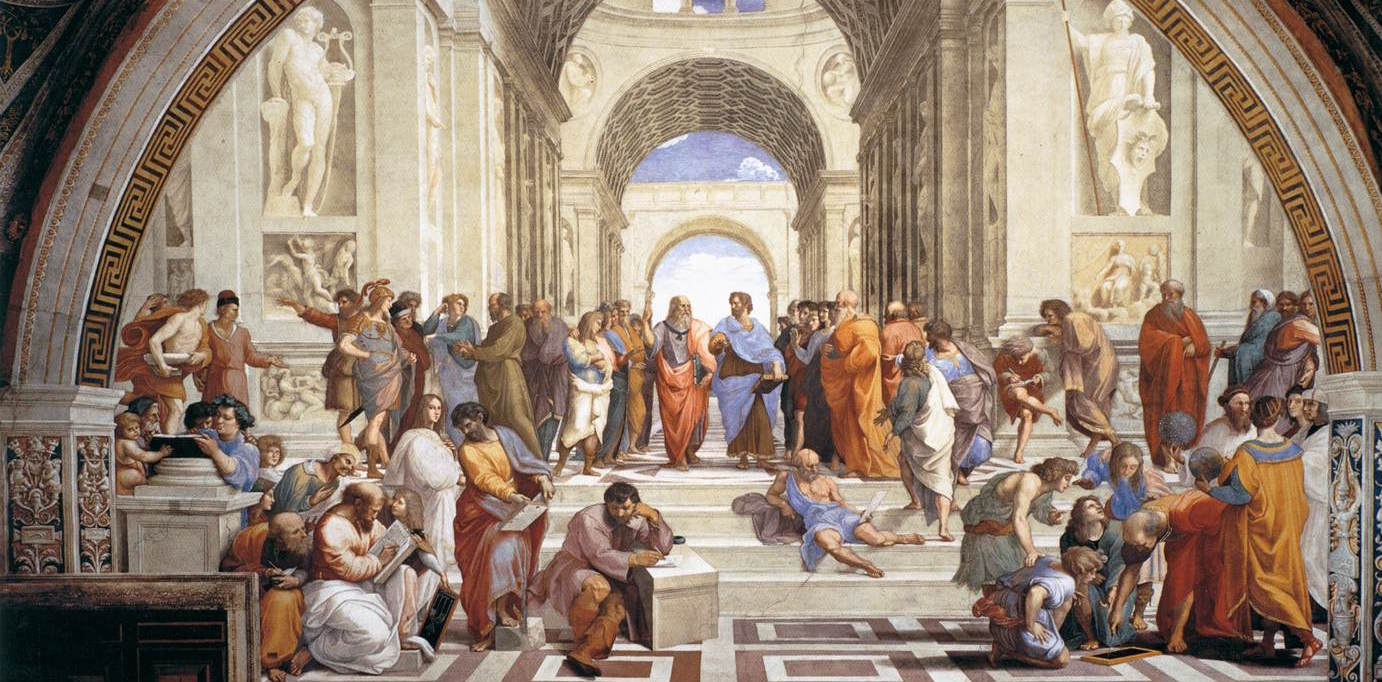
\includegraphics[scale=1.0]{img/the-school-of-athens.eps}
 \caption{拉斐尔《雅典学院》局部}
 \label{fig:the-school-of-athens}
\end{figure}
%\end{wrapfigure}

你也许注意到了本章第一节中,每个自然段的开头的第一个汉字连起来是“自然数产生”,我希望用这种形式表达同构的美。亚里士多德说美的主要形式就是秩序、匀称和确定性,这些正是数学研究的原则。我们用公理系统展示,自然数可以和几何同样建立在五条公理组成的大厦上。我们用自然数和列表的同构同样想表达这种形式上的美。文艺复兴时期的艺术大师拉斐尔在创作不朽的作品《雅典学院》时,也采用了同构,画中的历史人物和当时的人物对应。画面中心面向我们走来的是两位伟大学者的柏拉图和亚里士多德,其中柏拉图的原型是达芬奇,亚里士多德的原型是朱利亚诺$\cdot$达$\cdot$桑加洛。他们都是文艺复兴时期的伟大艺术家。画中的柏拉图右手向上指,意思是说人类应该思考永恒。而亚里士多德手向前伸,意思是说人类应该研究世界。这两个对立的手势,表达了他们思想上的分歧。中间台阶下方,倚箱沉思的是古希腊杰出的哲学家赫拉克利特,他是西方最早提出朴素辩证法和唯物论的卓越代表。他的原型是文艺复兴时期的另一位大师米开朗基罗。画面左前方以毕达哥拉斯为中心,他正在专注地书写。毕达哥拉斯右侧有一位身穿白色斗篷的金发青年,被认为是弗朗西斯柯·德拉·罗斐尔,他是乌尔宾诺未来的大公。画面右下方中心是手拿圆规的欧几里得(一说为阿基米德),他的周围有手持天球的天文学家托勒密,对面是画家拉斐尔的同乡、建筑家布拉曼特,而最边上那个头戴白帽的人,正是画家索多玛,上面露出半个脑袋、头戴深色圆形软帽的青年,就是画家拉斐本人。这让人联想起了伟大的音乐家巴赫把自己的名字B-A-C-H通过调式写进了《赋格的艺术》的音乐当中。《雅典学院》通过回忆历史上的黄金时代,表达人类对智慧和真理的追求,同时通过使用文艺复兴时期的人物作为原型,呼应了复兴古希腊艺术和哲学的思想的时代主题。这是形式与内容,结构与思想的多重同构。

\ifx\wholebook\relax \else
\begin{thebibliography}{99}

\bibitem{wiki-number}
Wikipedia. ``古代计数系统的历史''. \url{https://en.wikipedia.org/wiki/History_of_ancient_numeral_systems}

\bibitem{trip-to-number-kindom}
[美]卡尔文$\cdot$C$\cdot$克劳森. ``数学旅行家:漫游数王国''. 袁向东、袁钧译,上海教育出版社。ISBN:

\bibitem{wiki-babylonian-num}
Wikipedia. ``古巴比伦数字''. \url{https://en.wikipedia.org/wiki/Babylonian_numerals}

\bibitem{GEB}
[美]候世达 ``哥德尔、埃舍尔、巴赫——集异壁之大成''. 商务印书馆 1996. ISBN: 978-7-100-01323-9

\bibitem{Bird97}
Richard Bird, Oege de Moor. ``Algebra of Programming''. Univerisity of Oxford, Prentice Hall Europe. 1997. ISBN: 0-13-507245-X.

\bibitem{Gusen2014}
顾森 ``浴缸里的惊叹''. 人民邮电出版社. 2014, ISBN: 9787115355744

\end{thebibliography}

\expandafter\enddocument
%\end{document}

\fi
